\documentclass{article}
\usepackage[margin=1in]{geometry}
\usepackage[linesnumbered,ruled,vlined]{algorithm2e}
\usepackage{amsfonts}
\usepackage{amsmath}
\usepackage{amssymb}
\usepackage{amsthm}
\usepackage{enumitem}
\usepackage{fancyhdr}
\usepackage{hyperref}
\usepackage{minted}
\usepackage{multicol}
\usepackage{pdfpages}
\usepackage{standalone}
\usepackage[many]{tcolorbox}
\usepackage{tikz-cd}
\usepackage{transparent}
\usepackage{xcolor}
% \tcbuselibrary{minted}

\author{Nathan Solomon}

\newcommand{\fig}[1]{
    \begin{center}
        \includegraphics[width=\textwidth]{#1}
    \end{center}
}

% Math commands
\renewcommand{\d}{\mathrm{d}}
\DeclareMathOperator{\id}{id}
\DeclareMathOperator{\im}{im}
\DeclareMathOperator{\proj}{proj}
\DeclareMathOperator{\Span}{span}
\DeclareMathOperator{\Tr}{Tr}
\DeclareMathOperator{\tr}{tr}
\DeclareMathOperator{\ad}{ad}
\DeclareMathOperator{\ord}{ord}
%%%%%%%%%%%%%%% \DeclareMathOperator{\sgn}{sgn}
\DeclareMathOperator{\Aut}{Aut}
\DeclareMathOperator{\Inn}{Inn}
\DeclareMathOperator{\Out}{Out}
\DeclareMathOperator{\stab}{stab}

\newcommand{\N}{\ensuremath{\mathbb{N}}}
\newcommand{\Z}{\ensuremath{\mathbb{Z}}}
\newcommand{\Q}{\ensuremath{\mathbb{Q}}}
\newcommand{\R}{\ensuremath{\mathbb{R}}}
\newcommand{\C}{\ensuremath{\mathbb{C}}}
\renewcommand{\H}{\ensuremath{\mathbb{H}}}
\newcommand{\F}{\ensuremath{\mathbb{F}}}

\newcommand{\E}{\ensuremath{\mathbb{E}}}
\renewcommand{\P}{\ensuremath{\mathbb{P}}}

\newcommand{\es}{\ensuremath{\varnothing}}
\newcommand{\inv}{\ensuremath{^{-1}}}
\newcommand{\eps}{\ensuremath{\varepsilon}}
\newcommand{\del}{\ensuremath{\partial}}
\renewcommand{\a}{\ensuremath{\alpha}}

\newcommand{\abs}[1]{\ensuremath{\left\lvert #1 \right\rvert}}
\newcommand{\norm}[1]{\ensuremath{\left\lVert #1\right\rVert}}
\newcommand{\mean}[1]{\ensuremath{\left\langle #1 \right\rangle}}
\newcommand{\floor}[1]{\ensuremath{\left\lfloor #1 \right\rfloor}}
\newcommand{\ceil}[1]{\ensuremath{\left\lceil #1 \right\rceil}}
\newcommand{\bra}[1]{\ensuremath{\left\langle #1 \right\rvert}}
\newcommand{\ket}[1]{\ensuremath{\left\lvert #1 \right\rangle}}
\newcommand{\braket}[2]{\ensuremath{\left.\left\langle #1\right\vert #2 \right\rangle}}

\newcommand{\catname}[1]{{\normalfont\textbf{#1}}}

\newcommand{\up}{\ensuremath{\uparrow}}
\newcommand{\down}{\ensuremath{\downarrow}}

% Custom environments
\newtheorem{thm}{Theorem}[section]

\definecolor{probBackgroundColor}{RGB}{250,240,240}
\definecolor{probAccentColor}{RGB}{140,40,0}
\newenvironment{prob}{
    \stepcounter{thm}
    \begin{tcolorbox}[
        boxrule=1pt,
        sharp corners,
        colback=probBackgroundColor,
        colframe=probAccentColor,
        borderline west={4pt}{0pt}{probAccentColor},
        breakable
    ]
    \color{probAccentColor}\textbf{Problem \thethm.} \color{black}
} {
    \end{tcolorbox}
}

\definecolor{exampleBackgroundColor}{RGB}{212,232,246}
\newenvironment{example}{
    \stepcounter{thm}
    \begin{tcolorbox}[
      boxrule=1pt,
      sharp corners,
      colback=exampleBackgroundColor,
      breakable
    ]
    \textbf{Example \thethm.}
} {
    \end{tcolorbox}
}

\definecolor{propBackgroundColor}{RGB}{255,245,220}
\definecolor{propAccentColor}{RGB}{150,100,0}
\newenvironment{prop}{
    \stepcounter{thm}
    \begin{tcolorbox}[
        boxrule=1pt,
        sharp corners,
        colback=propBackgroundColor,
        colframe=propAccentColor,
        breakable
    ]
    \color{propAccentColor}\textbf{Proposition \thethm. }\color{black}
} {
    \end{tcolorbox}
}

\definecolor{thmBackgroundColor}{RGB}{235,225,245}
\definecolor{thmAccentColor}{RGB}{50,0,100}
\renewenvironment{thm}{
    \stepcounter{thm}
    \begin{tcolorbox}[
        boxrule=1pt,
        sharp corners,
        colback=thmBackgroundColor,
        colframe=thmAccentColor,
        breakable
    ]
    \color{thmAccentColor}\textbf{Theorem \thethm. }\color{black}
} {
    \end{tcolorbox}
}

\definecolor{corBackgroundColor}{RGB}{240,250,250}
\definecolor{corAccentColor}{RGB}{50,100,100}
\newenvironment{cor}{
    \stepcounter{thm}
    \begin{tcolorbox}[
        enhanced,
        boxrule=0pt,
        frame hidden,
        sharp corners,
        colback=corBackgroundColor,
        borderline west={4pt}{0pt}{corAccentColor},
        breakable
    ]
    \color{corAccentColor}\textbf{Corollary \thethm. }\color{black}
} {
    \end{tcolorbox}
}

\definecolor{lemBackgroundColor}{RGB}{255,245,235}
\definecolor{lemAccentColor}{RGB}{250,125,0}
\newenvironment{lem}{
    \stepcounter{thm}
    \begin{tcolorbox}[
        enhanced,
        boxrule=0pt,
        frame hidden,
        sharp corners,
        colback=lemBackgroundColor,
        borderline west={4pt}{0pt}{lemAccentColor},
        breakable
    ]
    \color{lemAccentColor}\textbf{Lemma \thethm. }\color{black}
} {
    \end{tcolorbox}
}

\definecolor{proofBackgroundColor}{RGB}{255,255,255}
\definecolor{proofAccentColor}{RGB}{80,80,80}
\renewenvironment{proof}{
    \begin{tcolorbox}[
        enhanced,
        boxrule=1pt,
        sharp corners,
        colback=proofBackgroundColor,
        colframe=proofAccentColor,
        borderline west={4pt}{0pt}{proofAccentColor},
        breakable
    ]
    \color{proofAccentColor}\emph{\textbf{Proof. }}\color{black}
} {
    \qed \end{tcolorbox}
}

\definecolor{noteBackgroundColor}{RGB}{240,250,240}
\definecolor{noteAccentColor}{RGB}{30,130,30}
\newenvironment{note}{
    \begin{tcolorbox}[
        enhanced,
        boxrule=0pt,
        frame hidden,
        sharp corners,
        colback=noteBackgroundColor,
        borderline west={4pt}{0pt}{noteAccentColor},
        breakable
    ]
    \color{noteAccentColor}\textbf{Note. }\color{black}
} {
    \end{tcolorbox}
}


\fancyhf{}
\setlength{\headheight}{24pt}

\date{\today}
\title{Math 182 Homework \#1}

\begin{document}
\maketitle

\begin{prob}
\end{prob}
\begin{enumerate}[label=(\alph*)]
    \item Suppose $a>0$ and $f(n) \in O(g(n))$. Then there exist positive numbers $C, N$ such that $f(n) \leq C g(n)$ whenever $n \geq N$. Since $a$ is positive, that means $f(n)^a \leq C^a g(n)^a$ whenever $n \geq N$, and $C^a$ is positive, so $f(n)^a \in O(g(n)^a)$.
    \item \begin{align*}
            \log(n!) &= \log \left( \prod_{k=1}^n k \right) \\
                     &= \sum_{k=1}^n \log(k) \\
                     &\leq \sum_{k=1}^n \log(n) \\
                     &= n \log(n),
    \end{align*}
    so $\log(n!)$ is also in $O(n \log(n))$. I also need to show that $\log(n!) \in \Omega(n \log(n))$: \begin{align*}
            \log(n!) &= \log \left( \prod_{k=1}^n k \right) \\
                     &= \sum_{k=1}^n \log(k) \\
                     &\geq \sum_{k=\ceil{n/2}}^n \log(k) \\
                     &\geq \sum_{k=\ceil{n/2}}^n \log(\floor{n/2}) \\
                     &= \floor{n/2} \log(\floor{n/2}) \\
                     &\in \Omega \left( \frac{n}{2} \log \left( \frac{n}{2} \right) \right) \\
                     &= \Omega \left( n (\log(n)-\log(2)) \right) \\
                     &= \Omega \left( n \log(n) \right).
    \end{align*}
    Since $\log(n!)$ is in both $O(n \log(n))$ and $\Omega(n \log(n))$, it is in $\Theta(n \log(n))$.
\item Suppose there is a degree $k$ polynomial $p(n)$ such that $n^{\log(n)} \in O(p(n))$. Then $n^{\log(n)} \in O(n^k)$, which means there is are positive constants $C, N$ such that $n^{\log(n)} \leq C n^k$ whenever $n \geq N$. This implies $\log(n) \leq k + \log_n(C)$ for all $n \geq N$, and that inequality can be rewritten as $\log(n)^2 \leq k \log(n) + \log(C)$. However, if $\log(n)$ is increased enough, that inequality will no longer be true, which contradicts my earlier statement that it is true for any $n \geq N$. Therefore $n \log(n) \not\in O(p(n))$.
\end{enumerate}

\bigskip
\par
\begin{prob}
\end{prob}
\begin{enumerate}[label=(\alph*)]
    \item If $n \leq 1$ then Foo(n) takes $f(1)=1$ step, otherwise it takes $f(n)=2f(n-1)+1$ steps. By induction, $f$ increases faster than $2^n$, which means for large $n$, the ``+1" in that formula becomes relatively insignificant. Therefore $f(n) \in \Theta(2^n)$.
    \item Assigning $1 \rightarrow x$ is one step, then the for loop repeats $n$ times. After the for loop, $x = (n^2+n)/2 \in \Theta(n^2)$, so the while loop repeats $\ceil{(n^2+n)/4}$ times. That means the total number of steps is $\Theta(n^2)$.
    \item The function $n \mapsto \floor{n/2}$ is equivalent to the right bitshift-by-one integer operator. The number of times you need to apply this to an integer in order to get to zero is equal to the number of digits in the binary representation of the integer, ignoring leading zeros, which is $\floor{\log_2(n)} \in \Theta(\log(n))$.
\end{enumerate}

\bigskip
\par
\begin{prob}
\end{prob}
\begin{enumerate}[label=(\alph*)]
    \item The only step that changes elements of the array is the swap command, so the integers in $A$ are only being reorganized, not changed. By induction, after running the inner ``for" loop, for each $k \leq i$, the $k$th element is less than or equal to all elements after it. Therefore, after the outer for loop is done, $A$ will be sorted in increasing order.
    \item By induction, after each step of the inner ``for" loop, $A[j+1]$ as a maximum element out of $A[1], A[2], \dots, A[j+1]$. Therefore, after each step of the outer ``for" loop, $A[n-i+1]$ will be a maximum element out of $A[1], A[2], \dots, A[n-i+1]$. Running the inner ``for" loop will not change elements $A[n-i+2], A[n-i+3], \dots, A[n]$, each of those elements will still be larger or equal to each previous element. Therefore, when the outer ``for" loop has finished, every element of the array will be larger or equal to each previous element.
\end{enumerate}

\bigskip
\par
\begin{prob}
\end{prob}
Note that I wrote my solution in Python, which is zero-indexed.
\begin{verbatim}
def bleh(A):
    n = len(A)
    r = 0
    i = 0
    j = 0
    while i < n and j < n:
        if A[i][j] == 0:
            i += 1
        else:
            r = i
            j += 1
    return r
\end{verbatim}
Each step of the ``while" loop runs in constant time and increases either $i$ or $j$ by one, which means the entire algorithms runs in $\Theta(n)$ time.

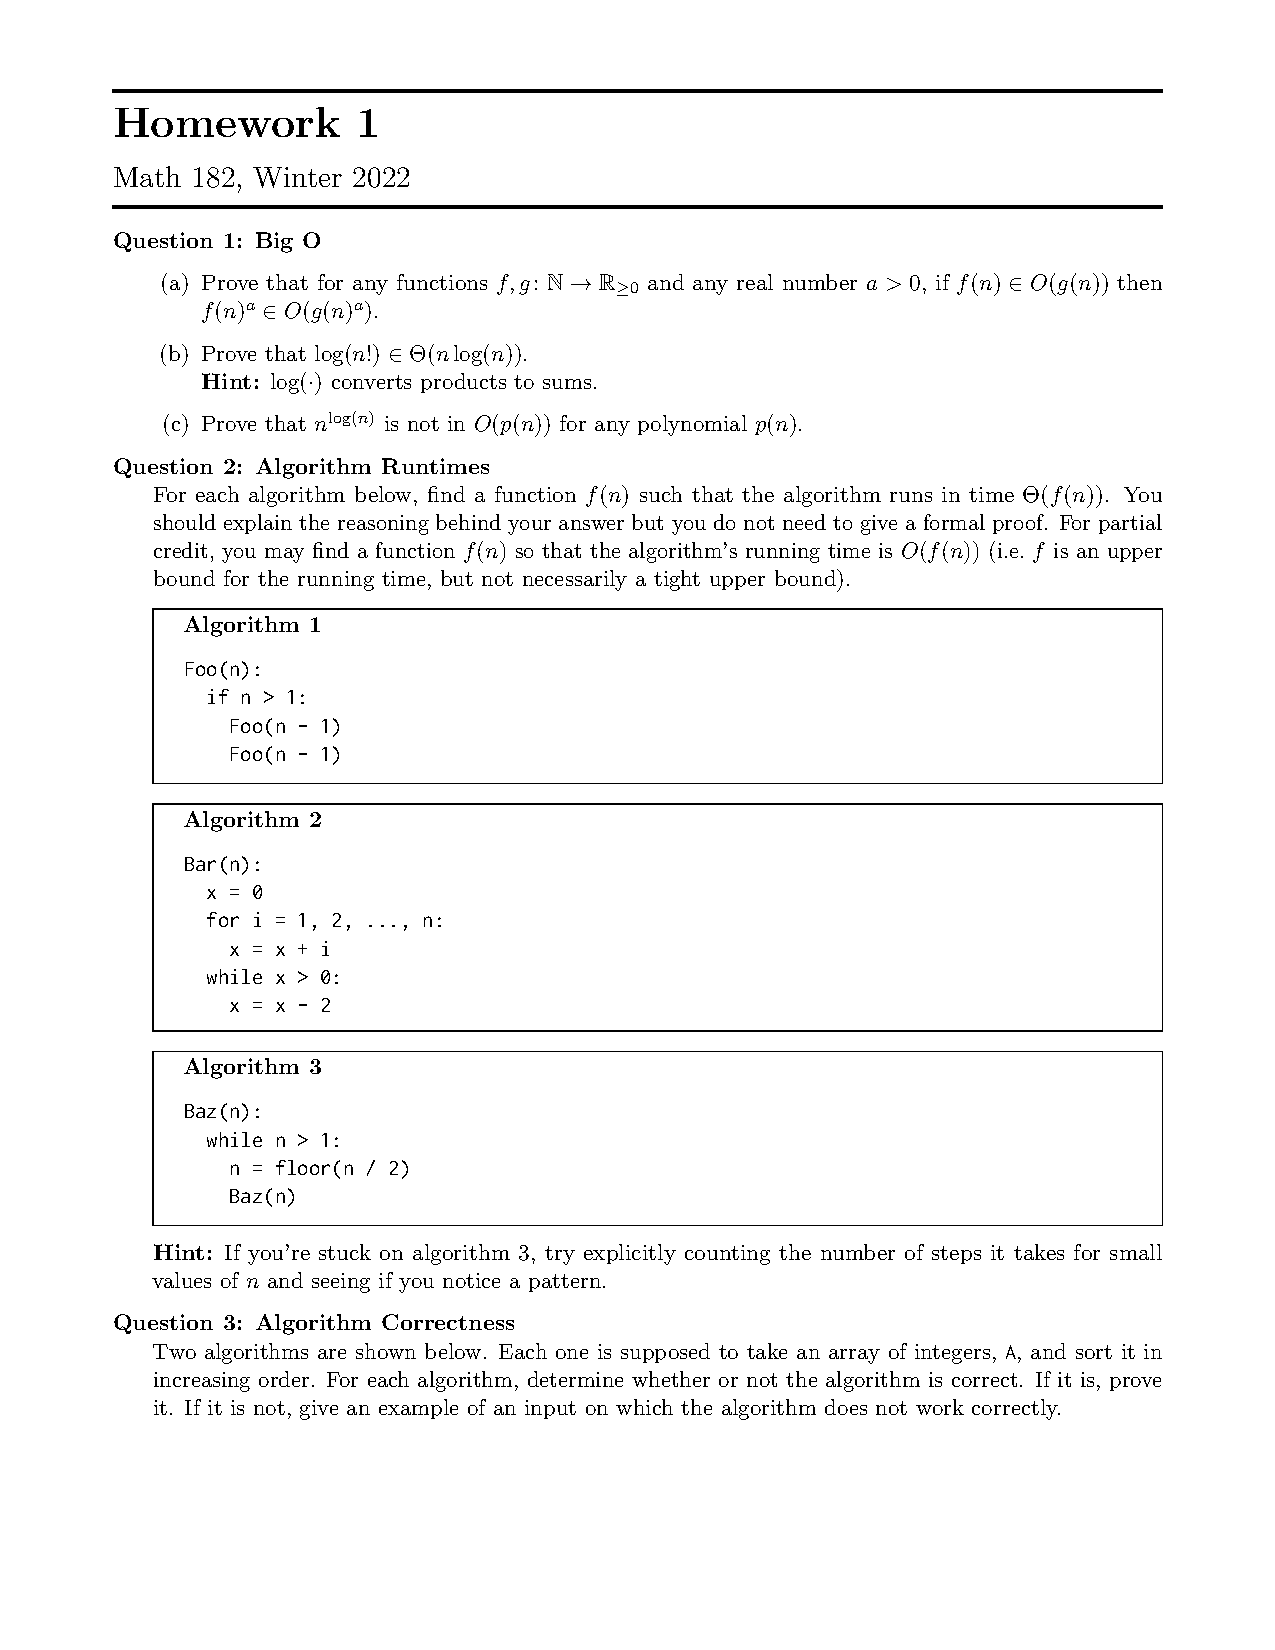
\includepdf[pages=-]{assignment.pdf}

\end{document}
